\documentclass[aspectratio=1610,bigger,utf8,xcolor=table]{beamer}
\usetheme{Hokie}
\usepackage{graphicx}
\usepackage[scaled]{berasans}
\usepackage[scaled]{beramono}
\usepackage[T1]{fontenc}
\usepackage{bibentry}
\usepackage{booktabs}
\usepackage{longtable}
\usepackage{subcaption}
\usepackage{tikz}
\nobibliography*
\logo{
\includegraphics[height=14pt]{2017-logo-color}}

\title{A Hybrid Micro-Tasking Framework for Event Coding}
\subtitle{Prelim Presentation}
\author{Sathappan Muthiah}
\institute{Virginia Tech}
\date{\today}
% \setlength{\tabcolsep}{4pt}
\usepackage{etoolbox}
\usetikzlibrary{arrows}


\usepackage{graphicx}

\usepackage{tikz}

%%%%%%%%%%%%%%%%%%%%%%%%%%%%%%%%%%%%%%%%%%%%%%%%%%%%%%%%%%%%%%%%%%%%%%
% LaTeX Overlay Generator - Annotated Figures v0.0.1
% Created with http://ff.cx/latex-overlay-generator/
% If this generator saves you time, consider donating 5,- EUR! :-)
%%%%%%%%%%%%%%%%%%%%%%%%%%%%%%%%%%%%%%%%%%%%%%%%%%%%%%%%%%%%%%%%%%%%%%
%\annotatedFigureBoxCustom{bottom-left}{top-right}{label}{label-position}{box-color}{label-color}{border-color}{text-color}
\newcommand*\annotatedFigureBoxCustom[8]{\draw[#5,thick,rounded corners] (#1) rectangle (#2);\node at (#4) [fill=#6,thick,shape=circle,draw=#7,inner sep=2pt,font=\sffamily,text=#8] {\textbf{#3}};}
%\annotatedFigureBox{bottom-left}{top-right}{label}{label-position}
\newcommand*\annotatedFigureBox[4]{\annotatedFigureBoxCustom{#1}{#2}{#3}{#4}{white}{white}{black}{black}}
\newcommand*\annotatedFigureText[4]{\node[draw=none, anchor=south west, text=#2, inner sep=0, text width=#3\linewidth,font=\sffamily] at (#1){#4};}
\newenvironment {annotatedFigure}[1]{\centering\begin{tikzpicture}
\node[anchor=south west,inner sep=0] (image) at (0,0) { #1};\begin{scope}[x={(image.south east)},y={(image.north west)}]}{\end{scope}\end{tikzpicture}}
%%%%%%%%%%%%%%%%%%%%%%%%%%%%%%%%%%%%%%%%%%%%%%%%%%%%%%%%%%%%%%%%%%%%%%


\makeatletter
\def\rowcolor{\noalign{\ifnum0=`}\fi\bmr@rowcolor}
\newcommand<>{\bmr@rowcolor}{%
    \alt#1%
        {\global\let\CT@do@color\CT@@do@color\@ifnextchar[\CT@rowa\CT@rowb}% 
        {\ifnum0=`{\fi}\@gooble@rowcolor}% 
}

\newcommand{\@gooble@rowcolor}[2][]{\@gooble@rowcolor@}
\newcommand{\@gooble@rowcolor@}[1][]{\@gooble@rowcolor@@}
\newcommand{\@gooble@rowcolor@@}[1][]{\ignorespaces}
\makeatother



\makeatletter
\def\cellcolor{{\ifnum0=`}\fi\bmr@cellcolor}
\newcommand<>{\bmr@cellcolor}{%
    \alt#1%
        {\global\let\CT@do@color\CT@@do@color\@ifnextchar[\CT@rowa\CT@rowb}% 
        {\ifnum0=`{\fi}\@gooble@cellcolor}% 
}

\newcommand{\@gooble@cellcolor}[2][]{\@gooble@cellcolor@}
\newcommand{\@gooble@cellcolor@}[1][]{\@gooble@cellcolor@@}
\newcommand{\@gooble@cellcolor@@}[1][]{\ignorespaces}
\makeatother

\makeatletter
\beamer@compresstrue
\patchcmd{\insertnavigation}{\hskip-1.875ex plus-1fill}{}{}{}
\apptocmd{\partentry}{\beamer@xpos=0\relax}{}{}
\def\sectionentry#1#2#3#4#5{% section number, section title, page
  \ifnum#5=\c@part%
  \hbox{\def\insertsectionhead{#2}%
    \def\insertsectionheadnumber{#1}%
    \def\insertpartheadnumber{#5}%
    {%
      \usebeamerfont{section in head/foot}\usebeamercolor[fg]{section in head/foot}%
      \ifnum\c@section=#1%
        \rlap{\hyperlink{Navigation#3}{{\usebeamertemplate{section in head/foot}}}}%
      \fi}%
  }%
  \fi\ignorespaces}
\makeatother
\begin{document}

\AtBeginSection[]{
  \begin{frame}
  \vfill
  \centering
  \begin{beamercolorbox}[sep=8pt,center,shadow=true,rounded=true]{title}
    \usebeamerfont{title}\insertsectionhead\par%
  \end{beamercolorbox}
  \vfill
  \end{frame}
}


\addtobeamertemplate{navigation symbols}{}{%
    \usebeamerfont{footline}%
    \usebeamercolor[fg]{footline}%
    \hspace{1em}%
    \insertframenumber/\inserttotalframenumber
}

\tikzstyle{every picture}+=[remember picture]

% By default all math in TikZ nodes are set in inline mode. Change this to
% displaystyle so that we don't get small fractions.
\everymath{\displaystyle}

% \AtBeginSection[]
% {
% \begin{frame}<beamer>{\insertsectionhead}
% \tableofcontents[currentsection,currentsubsection, 
%     hideothersubsections
% ]
% \end{frame}
% }

\frame{\titlepage}

\begin{frame}
	\frametitle{Contents}
	\tableofcontents[hideallsubsections]
\end{frame}


\section{Introduction}
% \subsection{what is an Event}
\begin{frame}{Introduction}
\begin{block}{What is an Event of Interest?}
 Any significant societal event  that happened in the recent past and is reported in a national news paper of repute. Societal events of interest include \textit{Military Action}, \textit{Non-state Actor} and \textit{Civil Unrest} events. 
\end{block}
\pause
\begin{block}{Structured Event Record}
An event record generally contains information regarding: 
\begin{itemize}
    \item \textbf{\textit{Who}} is responsible for the event
    \item \textbf{\textit{When}} the event happened
    \item \textbf{\textit{Where}} did the event occur
    \item \textbf{\textit{Why}} did the event occur
    \item \textbf{\textit{What}} kind of event occured
\end{itemize}
\end{block}
\end{frame}

% \subsection{Example}
\begin{frame}{Example}

\tikzstyle{na} = [baseline=-.5ex]

\begin{itemize}[<+-| alert@+>]
    \item \textbf{Who}
        \tikz[na] \node[coordinate] (n1) {};
\end{itemize}

\begin{block}{}
Beirut, Lebanon \tikz[baseline]{ \node[fill=blue!20,anchor=base] (t4){2:00 A.M.};}.In addition to the arrival of Syrian military reinforcements, \tikz[baseline]{\node[fill=red!20,anchor=base] (t1) {the Russian Aerospace forces};} have been 
\tikz[baseline]{\node[fill=black!20,anchor=base] (t2) {repeatedly pounding};} the \tikz[baseline]{
\node[fill=green!20,anchor=base] (t3) {Jisr Al-Shughour countryside};}, forcing the jihadist rebels of \tikz[baseline]{
            \node[fill=red!20,anchor=base] (t1) {Turkestan Islamic Party (TIP)};} to abandon several outposts.
\end{block}

\begin{itemize}[<+-| alert@+>]
    \item \textbf{Where}
        \tikz[na]\node [coordinate] (n2) {};
    \item \textbf{When}
        \tikz[na]\node [coordinate] (n4) {};
    \item \textbf{What}
    \tikz[na]\node [coordinate] (n3) {};
\end{itemize}

% Now it's time to draw some edges between the global nodes. Note that we
% have to apply the 'overlay' style.
\begin{tikzpicture}[overlay]
        \path[->]<1-> (n1) [bend left] edge (t1);
        \path[->]<2-> (n2) [bend right] edge (t3);
        \path[->]<3-> (n3) edge [out=0, in=-90] (t2);
        \path[->]<4-> (n4) edge [out=0, in=-90] (t4);
\end{tikzpicture}

\end{frame}

% \subsection{Why track events?}
\begin{frame}{Why track/record events?}
\begin{itemize}
    \item Travel Alerts
    \item Supply chain management
    \item Prioritizing citizen grievances
    \item Design measures to control violence and minimize disruptions
    \item Relationships to market and government instability
\end{itemize}
\end{frame}

\section{Studying Model Drift in Anticipatory Intelligence Systems}
% \subsection{EMBERS Introduction}
\begin{frame}{Studying Model-drift in Anticipatory Intelligence Systems}
\begin{itemize}
    \item EMBERS Introduction
    \item EMBERS Performance
    \item Ablation Testing
    \item EMBERS Successes and Misses
    \item Uncertainty in forecasting
    \item Model Drift
\end{itemize}
    
\end{frame}
\begin{frame}{EMBERS Introduction}
EMBERS - Early Model Based Event Recognition using Surrogates
    \begin{itemize}
        \item 24x7 continuous forecasting system
        \item Deployed - Nov 2012 
        \item Aims to develop methods for continuous, automated analysis of publicly available data in order to anticipate and/or detect population-level events
        \item Event classes 
            \begin{itemize}
                \item Civil Unrest, Rare Diseases, Influenza Like Illness, Elections, Domestic Political Crises
            \end{itemize}
        \item ~\cite{kdd:beating-the-news, doyle2014forecasting, zhao2014unsupervised} ...
    \end{itemize}
\end{frame}

% \subsection{EMBERS Performance}
\begin{frame}{EMBERS Performance}
\begin{figure}
    \centering
    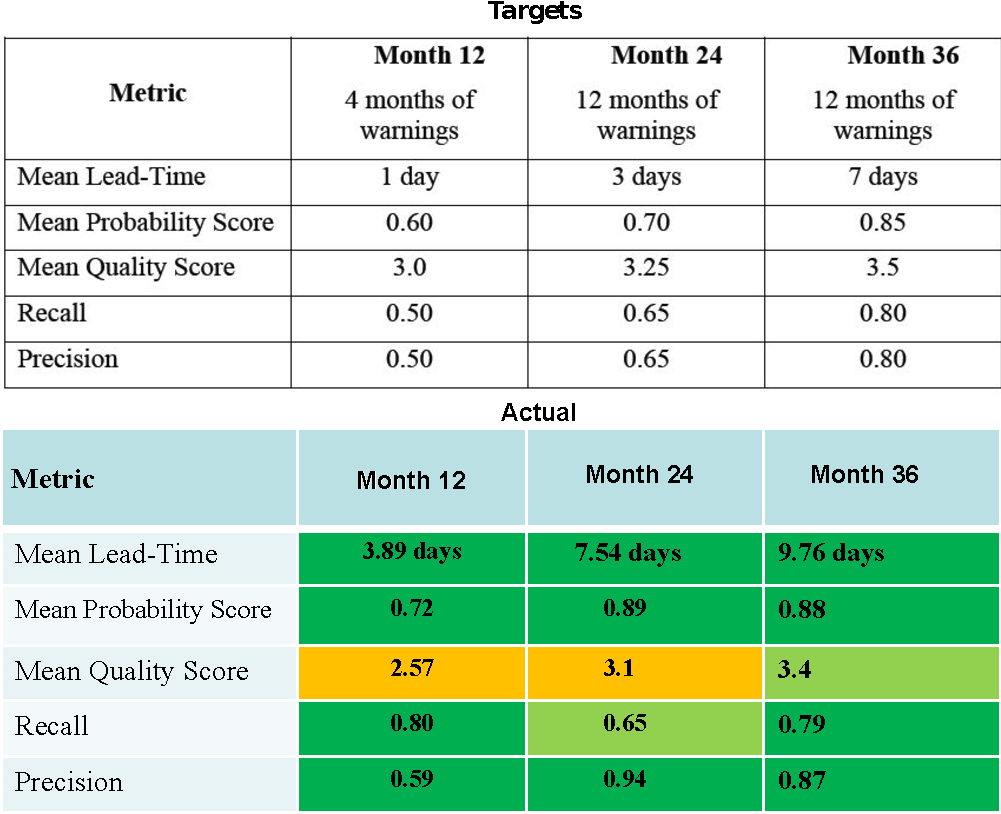
\includegraphics[width=0.7\textwidth]{Problem1/figures/performance_tb1.pdf}
    \label{fig:my_label}
\end{figure}
\end{frame}

\begin{frame}{EMBERS Introduction (Contd.)}
    Data Sources
    \begin{itemize}
        \item Social Media sources: Twitter, Facebook events
        \item Traditional Media: News, Blogs
        \item Historical events: ICEWS~\cite{boschee2015icews}, GDELT~\cite{leetaru2013gdelt}
        \item Numerical - Tor, stock/currency exchange values
    \end{itemize}
    
    % Models
    % \begin{itemize}
    %     \item Dynamic Query Expansion, Planned Protest, Volume based model, MLE, BaseRate etc
    % \end{itemize}
\end{frame}

% \subsection{Ablation Testing}
\begin{frame}{Ablation Testing}

\begin{table}
\resizebox{\columnwidth}{!}{
\begin{tabular}{l|cccc}
\toprule
Data Source          & Quality-Score & Lead-time & Precision & Recall \\
\midrule
Removing news and blogs & -16.48\% &-55\% &+35\% &-14\% \\

Removing social media & +8.42\% & +30\%  &+79\% &-33\% \\
\bottomrule
\end{tabular}
}
\end{table}

\pause
\begin{itemize}
    \item Social media sources provide high recall \pause
        \begin{itemize} 
            \item Daily chatter/discussion 
        \end{itemize}
    \item High lead-time from traditional sources \pause
        \begin{itemize}
            \item Planned Protests are generally reported in traditional media
        \end{itemize}
\end{itemize}
\end{frame}


% \subsection{EMBERS Successful forecasts}
\begin{frame}{Successful Forecasts}
\begin{center}
\small
    Paraguay Protests Feb. 2015
\end{center}
\vspace{-1em}

\begin{tikzpicture}
\begin{scope}[xshift=6cm]
    \node[anchor=south west,inner sep=0] (image) at (0,0) {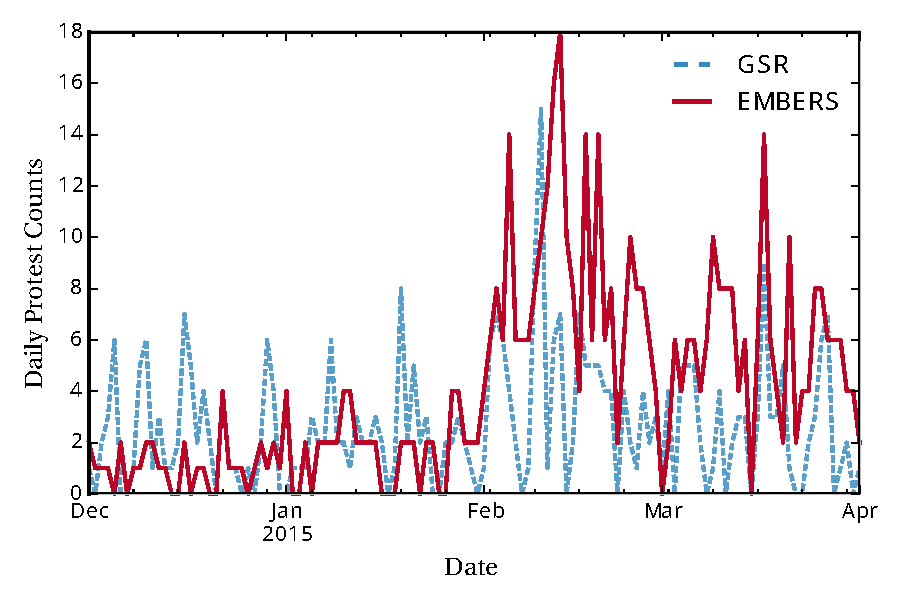
\includegraphics[width=0.5\textwidth]{Problem1/figures/paraguayFeb15.pdf}};
    \begin{scope}[x={(image.south east)},y={(image.north west)}]
        % \draw[red,ultra thick] (0.48,0.80) ellipse (0.55,0.95);
        \draw[green,ultra thick] (0.6,0.50) ellipse (1cm and 2cm) node(peak){};
    \end{scope}
\end{scope}
\node [anchor=west] (note) at (1,3) {{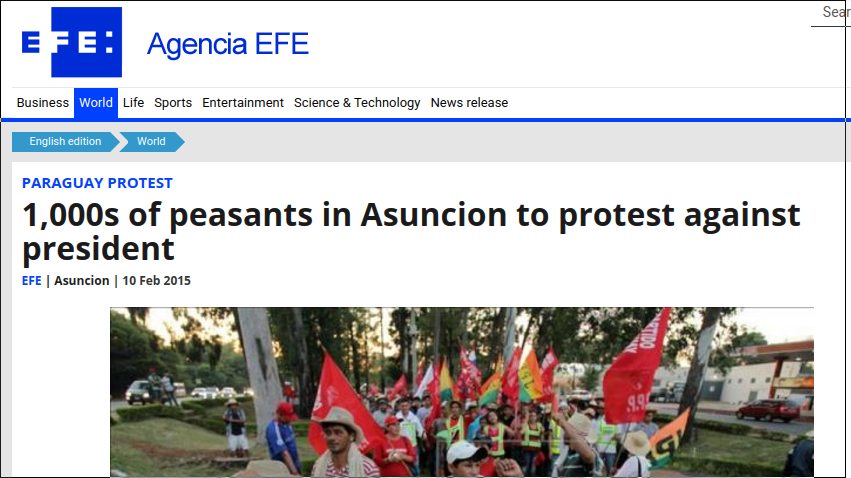
\includegraphics[width=0.3\textwidth]{Problem1/figures/peasants.png}};};

\path[->,green,thick] (note) edge [bend right] (peak);
\end{tikzpicture}%
\vspace{-1em}
\pause

Some more examples:
\begin{itemize}
\small
    \item Brazilian Spring (June 2013)
    \item Venezuelan Protests (Feb-March 2014)
    \item Mexico (Oct 2014)
    \item Colombia (Dec'14-March 2015)
\end{itemize}
\end{frame}


% \begin{frame}{Frame Title}
    
% % \begin{figure}[h!t]

% % \begin{annotatedFigure}
% % 	{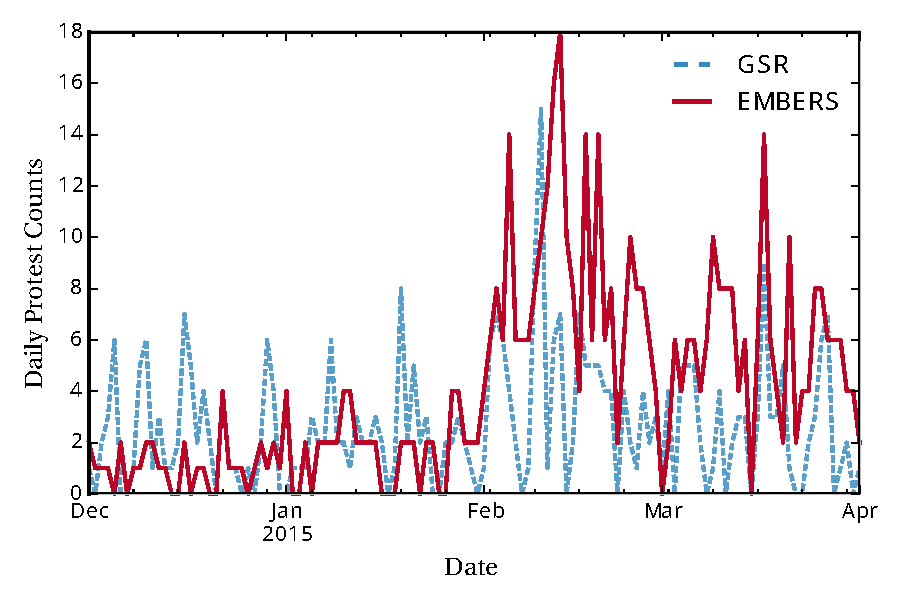
\includegraphics[width=0.8\linewidth]{Problem1/figures/paraguayFeb15.pdf}}\pause
% % 	\annotatedFigureBox{0.4995,0.2514}{0.731,0.9505}{A}{0.4995,0.2514}%bl
% % \end{annotatedFigure}

% % \end{figure}

% \begin{tikzpicture}
% \begin{scope}[xshift=1.5cm]
%     \node[anchor=south west,inner sep=0] (image) at (0,0) {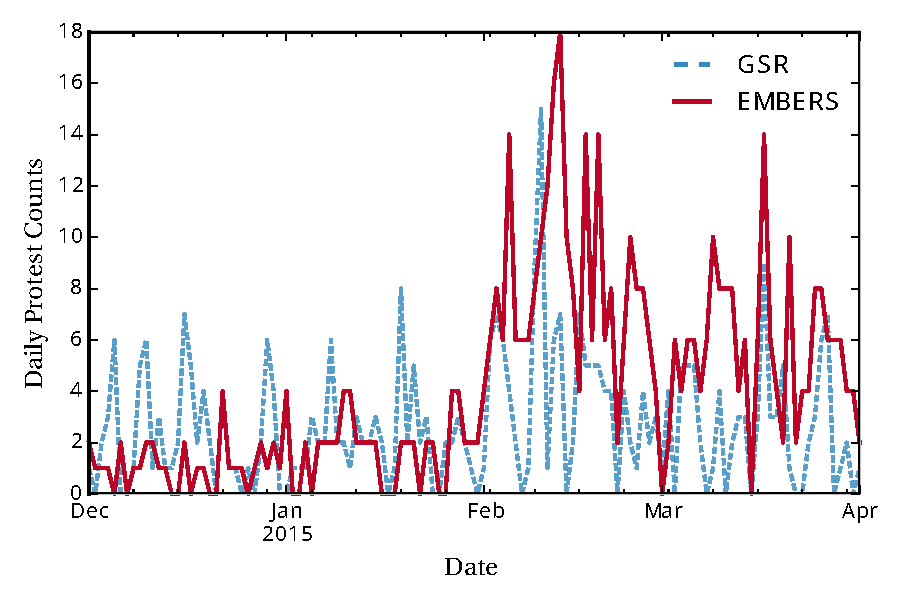
\includegraphics[width=0.5\textwidth]{Problem1/figures/paraguayFeb15.pdf}};
%     \begin{scope}[x={(image.south east)},y={(image.north west)}]
%         % \draw[red,ultra thick] (0.48,0.80) ellipse (0.55,0.95);
%         \draw[green,ultra thick] (0.6,0.50) ellipse (1cm and 4cm) node(peak){};
%     \end{scope}
% \end{scope}
% \node [anchor=west] (note) at (1,5) {{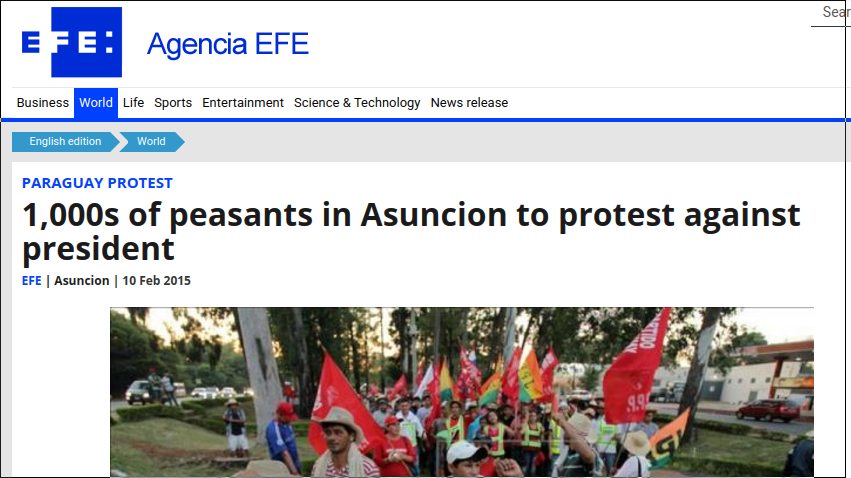
\includegraphics[width=0.3\textwidth]{Problem1/figures/peasants.png}};};

% \path[->,green,thick] (note) edge [bend right] (peak);
% \end{tikzpicture}%


% \end{frame}



% \subsection{EMBERS Misses}
\begin{frame}{EMBERS Misses}
\begin{center}
    Mexico 2014
\end{center}
    \begin{figure}
        \centering
        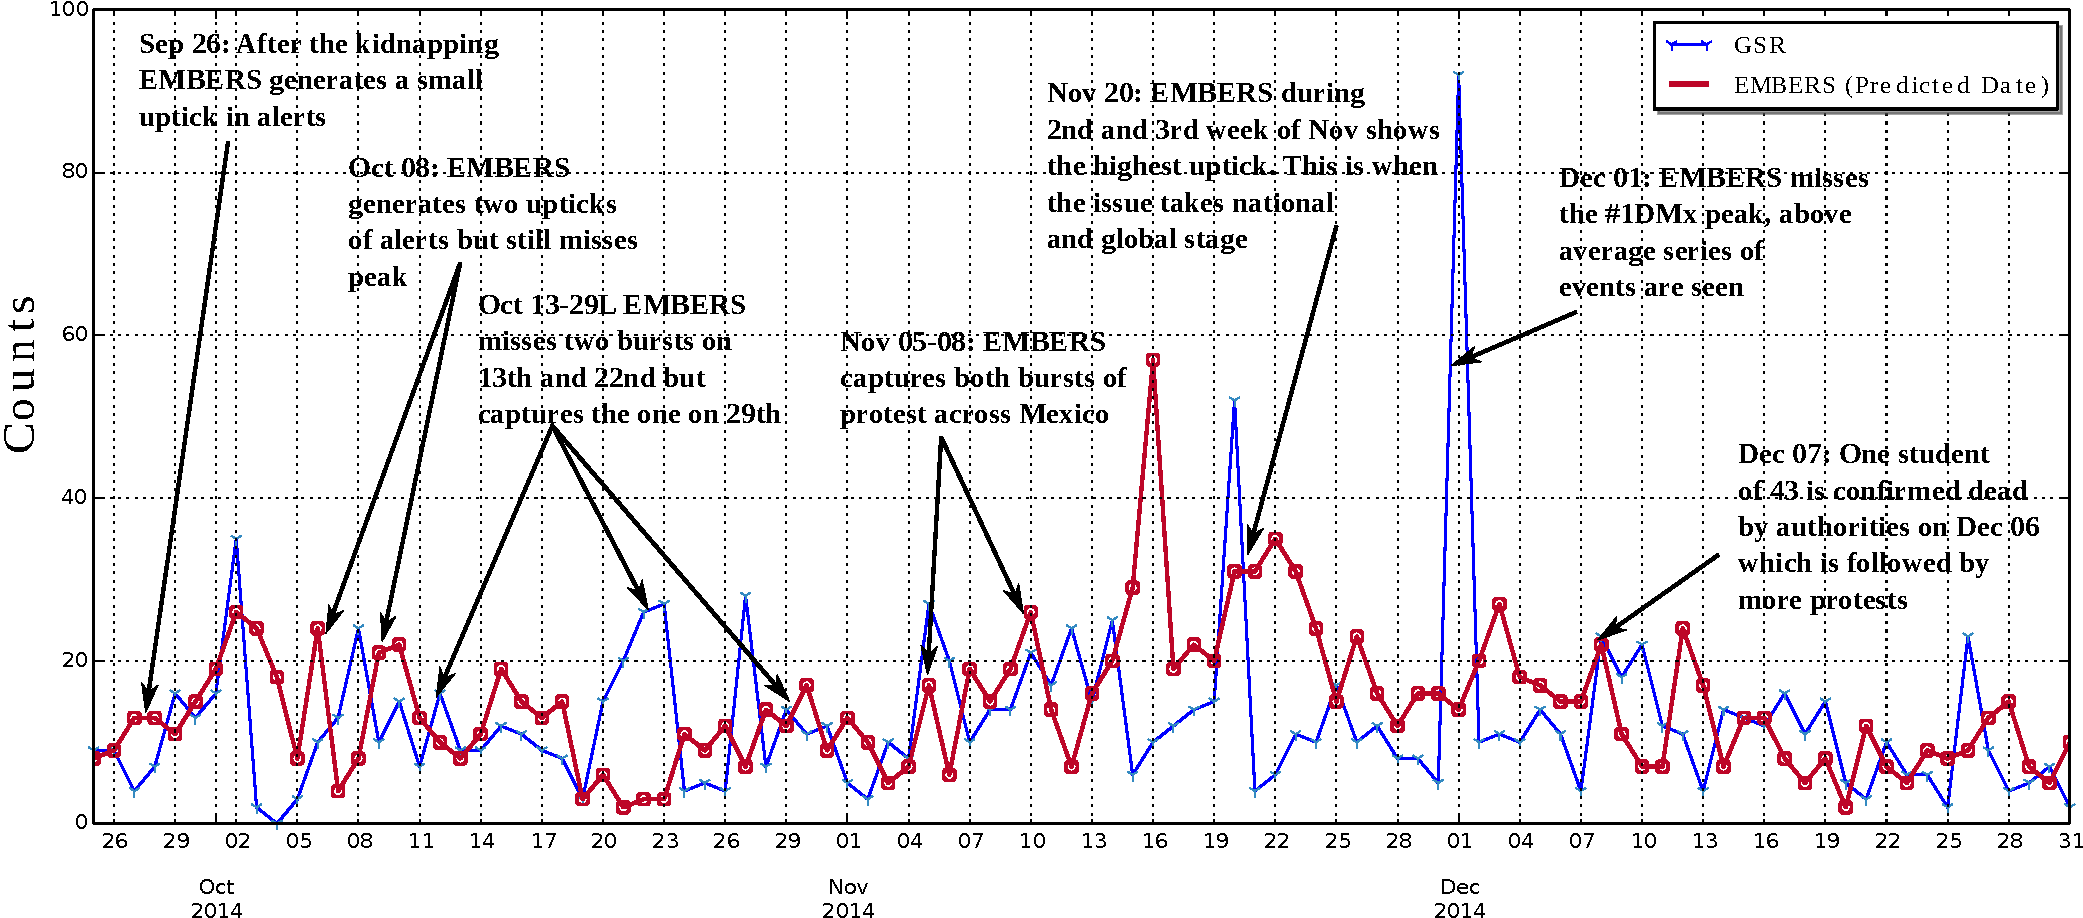
\includegraphics[width=\textwidth]{Problem1/figures/mx_timeline.pdf}
    \end{figure}
\end{frame}

% \subsection{Uncertainty in Forecasts}
   \begin{frame}{Uncertainty in Forecasting}
       
    \begin{figure}
        \centering
        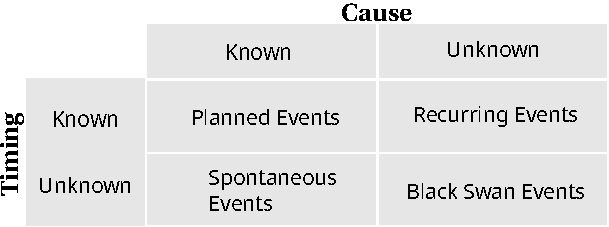
\includegraphics[width=\textwidth]{Problem1/figures/event_confusionMatrix.pdf}
    \end{figure}
    \end{frame}

% \subsection{Model Drift}
\begin{frame}{Model Drift}
\begin{figure}
    \centering
    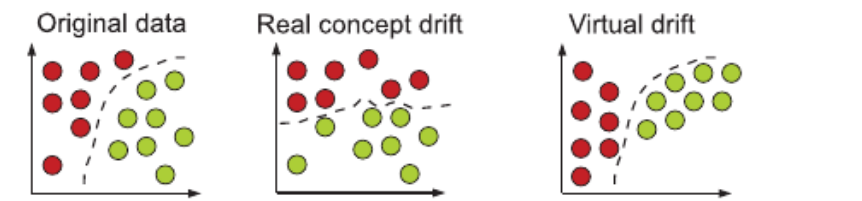
\includegraphics[width=0.9\textwidth]{Problem1/figures/modelDrift.png}
    \caption{Gama et al.,~\cite{gama2014survey}}
\end{figure}
\vspace{-1em}
Broadly defined as change in data-target relationship over time \\
Kinds of drift
\begin{itemize}
    \item \textit{Input(or Target) data drift}: only $P(x)$ changes not $P(y|x)$. Example-Change in twitter volume over time
    \item \textit{Input-Target Drift}: Relationship between input and target changes over time
\end{itemize}
\end{frame}


\begin{frame}{Model Drift in EMBERS}
Possible reasons
\begin{itemize}
    \item<1->Significant change in event landscape
    \begin{itemize}
        \item<2-> Change in rate of events 
        \only<2->{
                 \begin{figure}
                    \centering
                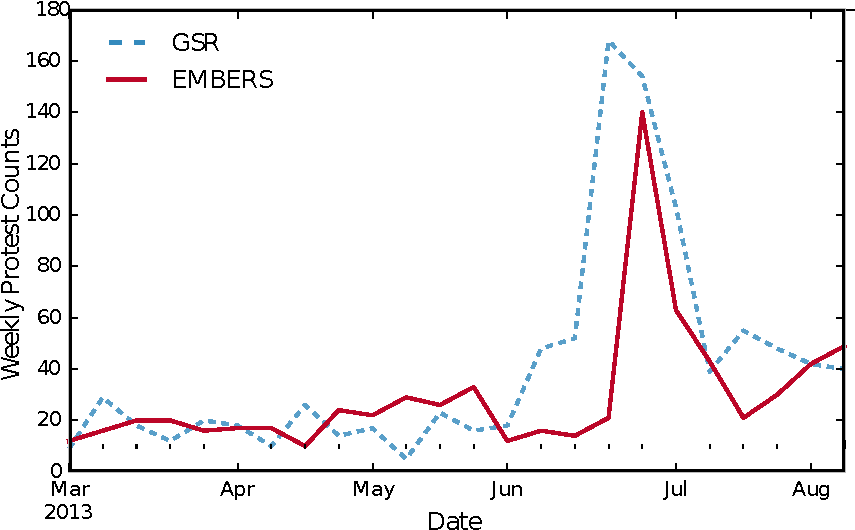
\includegraphics[width=0.5\textwidth]{Problem1/figures/brazilJune13.pdf}
                \end{figure}
                }
        % \item Example: Government instability can cause lead to increase in number of protests
    \end{itemize}
    \item<3-> Data sources becoming obsolete (or arrival of New data sources)
        \begin{itemize}
            \item Black swan events (unknown-unknowns)
        \end{itemize}
\end{itemize}
\end{frame}


\begin{frame}{Model drift Adaptation - Steps involved}
Three main steps:
\begin{itemize}
    \item Concept Drift Detector
    \begin{itemize}
        \item Near real-time source of GSR needed
            \begin{itemize}
                \item EMBERS AutoGSR~\cite{saraf2016embers}
            \end{itemize}
        \item HQCD~\cite{chakraborty2016hierarchical}, BOCPD~\cite{adams2007bayesian} etc
    \end{itemize} \pause
    \item Real-time Parameter tuning based on updated estimate of expected rate of events for time $t+1$
    \begin{itemize}
        \item Quality score threshold in EMBERS suppressor
            \begin{itemize}
                \item update threshold based on (1) estimated rate of events, (2) expected number of alerts and (3) suppressor quality score density distribution
            \end{itemize}\pause
        \item Rate-Adapted BaseRate
        \begin{itemize}
            \item Sample events at random from past month to account for difference in rate
        \end{itemize}
    \end{itemize}\pause
    \item Model re-training after enough data is accumulated from post-change distribution
\end{itemize}
    
\end{frame}

\subsection{Model drift Adaptation Framework}
\begin{frame}{Model drift Adaptation Framework}
    \begin{figure}
        \centering
        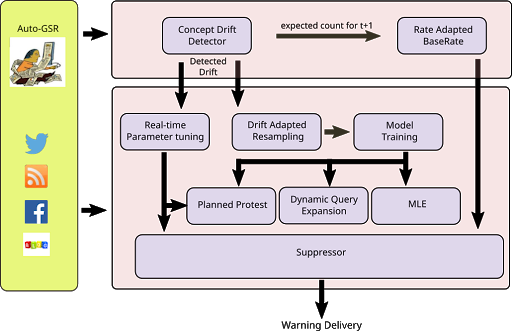
\includegraphics[width=0.8\textwidth]{Problem1/figures/driftAdaptationFramework.png}
    \end{figure}
\end{frame}

% \subsection{Model Drift Experiment settings}
\begin{frame}{Model drift Experiments}
\begin{itemize}
    \item \textbf{\textit{Monthly trained}}: All models for month `$n$' are trained with data upto `$n-1$'
    \item \textbf{\textit{6 months old}}: Models trained using data upto `$n-6$' data and no drift correction done
    \item \textit{\textbf{EMBERS delivered}}: Set of delivered EMBERS alerts
    \item \textit{\textbf{Drift Corrected}}: Models are adapted if and only if a drift is detected
\end{itemize}
\end{frame}




% \subsection{Model Drift Results}
\begin{frame}{Model Drift Results}
\vspace{-1em}
\begin{table}
\scriptsize
\begin{tabular}{p{1.5 cm}p{2cm}rrrrrrrrrrr}
\toprule
& & LS &  DS &  ES &  PS &  QS &  Prob-M &  LT &  Prec. &  Recall \\
\midrule
\textbf{Venezuela} &   Monthly Trained  & \textbf{0.90} &    0.94 &    0.58 &    \textbf{0.39} &   \textbf{ 3.69} &        \textbf{0.89} &    \textbf{5.01} &       \textbf{0.93} &    0.60 \\
         &      6 months old   & 0.88 &    0.94 &    \textbf{0.60} &    \textbf{0.39} &    3.64 &        0.88 &    2.93 &       0.92 &    0.49 \\
         &  EMBERS-delivered   & 0.88 &    \textbf{0.95} &    0.58 &    0.38 &    3.64 &        0.87 &    4.53 &       0.91 &    0.50 \\
         &   Drift Corrected   & 0.84 &    0.90 &    0.59 &    0.34 &    3.48 &        0.86 &    3.99 &       0.88 &    \textbf{0.75} \\
\midrule
\textbf{Brazil}   &   Monthly Trained   & 0.88 &    0.89 &    \textbf{0.48} &    0.42 &    3.54 &        0.73 &    \textbf{6.98} &       0.60 &    0.51 \\
         &      6 months old   & 0.86 &    0.87 &    0.46 &    0.49 &    3.46 &        \textbf{0.77} &    3.46 &       \textbf{0.75} &    0.37 \\
         &  EMBERS-delivered   & 0.87 &    0.88 &    0.47 &    \textbf{0.52} &    3.49 &        \textbf{0.77} &    5.89 &       0.73 &    0.51 \\
         &   Drift Corrected   &\textbf{0.89} &    \textbf{0.89} &    0.47 &    0.42 &    \textbf{3.55} &        0.76 &    5.27 &       0.66 &    \textbf{0.60} \\
\bottomrule
\end{tabular}
\end{table}

\begin{itemize}
\small
    \item Regular training shows higher lead-time
    \item Quality does not improve much with regular re-training
    \item Recall improves with regular re-training
    \item Drift correction helps improve recall with minor\\ sacrifice in precision (and QS w.r.t to venezuela)
\end{itemize}
\end{frame}

\begin{frame}{Takeaways}
\begin{itemize}
    \item Ground truth definition/ quality/ granularity(specificity) has big impact on model performance
    \item Single OSI source may be noisy/unreliable
    \item Model-drift is a major issue
        \begin{itemize}
            \item Near-real time source of Ground-Truth necessary for timely change detection
            \item Real-time parameter tuning necessary for updating models
        \end{itemize}
\end{itemize}
    
\end{frame}

\section{A Hybrid Micro Tasking Framework for Event Coding}
%\subsection{What is Event Coding}
\begin{frame}{A Hybrid Micro Tasking Framework for Event Coding}
Outline:
\begin{itemize}
    \item What is Event Coding?
    \item Necessity for a new Event Coder?
    \item System Framework
    \item Micro-tasks for Event Coding
\begin{itemize}
   \item Geo-coding
    \item Actor/Target Linking
    \item Temporal Resolution
    \item Event Detection
\end{itemize} 
    \item Performance
\end{itemize}
\end{frame}


\begin{frame}{What is Event Coding}
    \begin{figure}
        \centering
        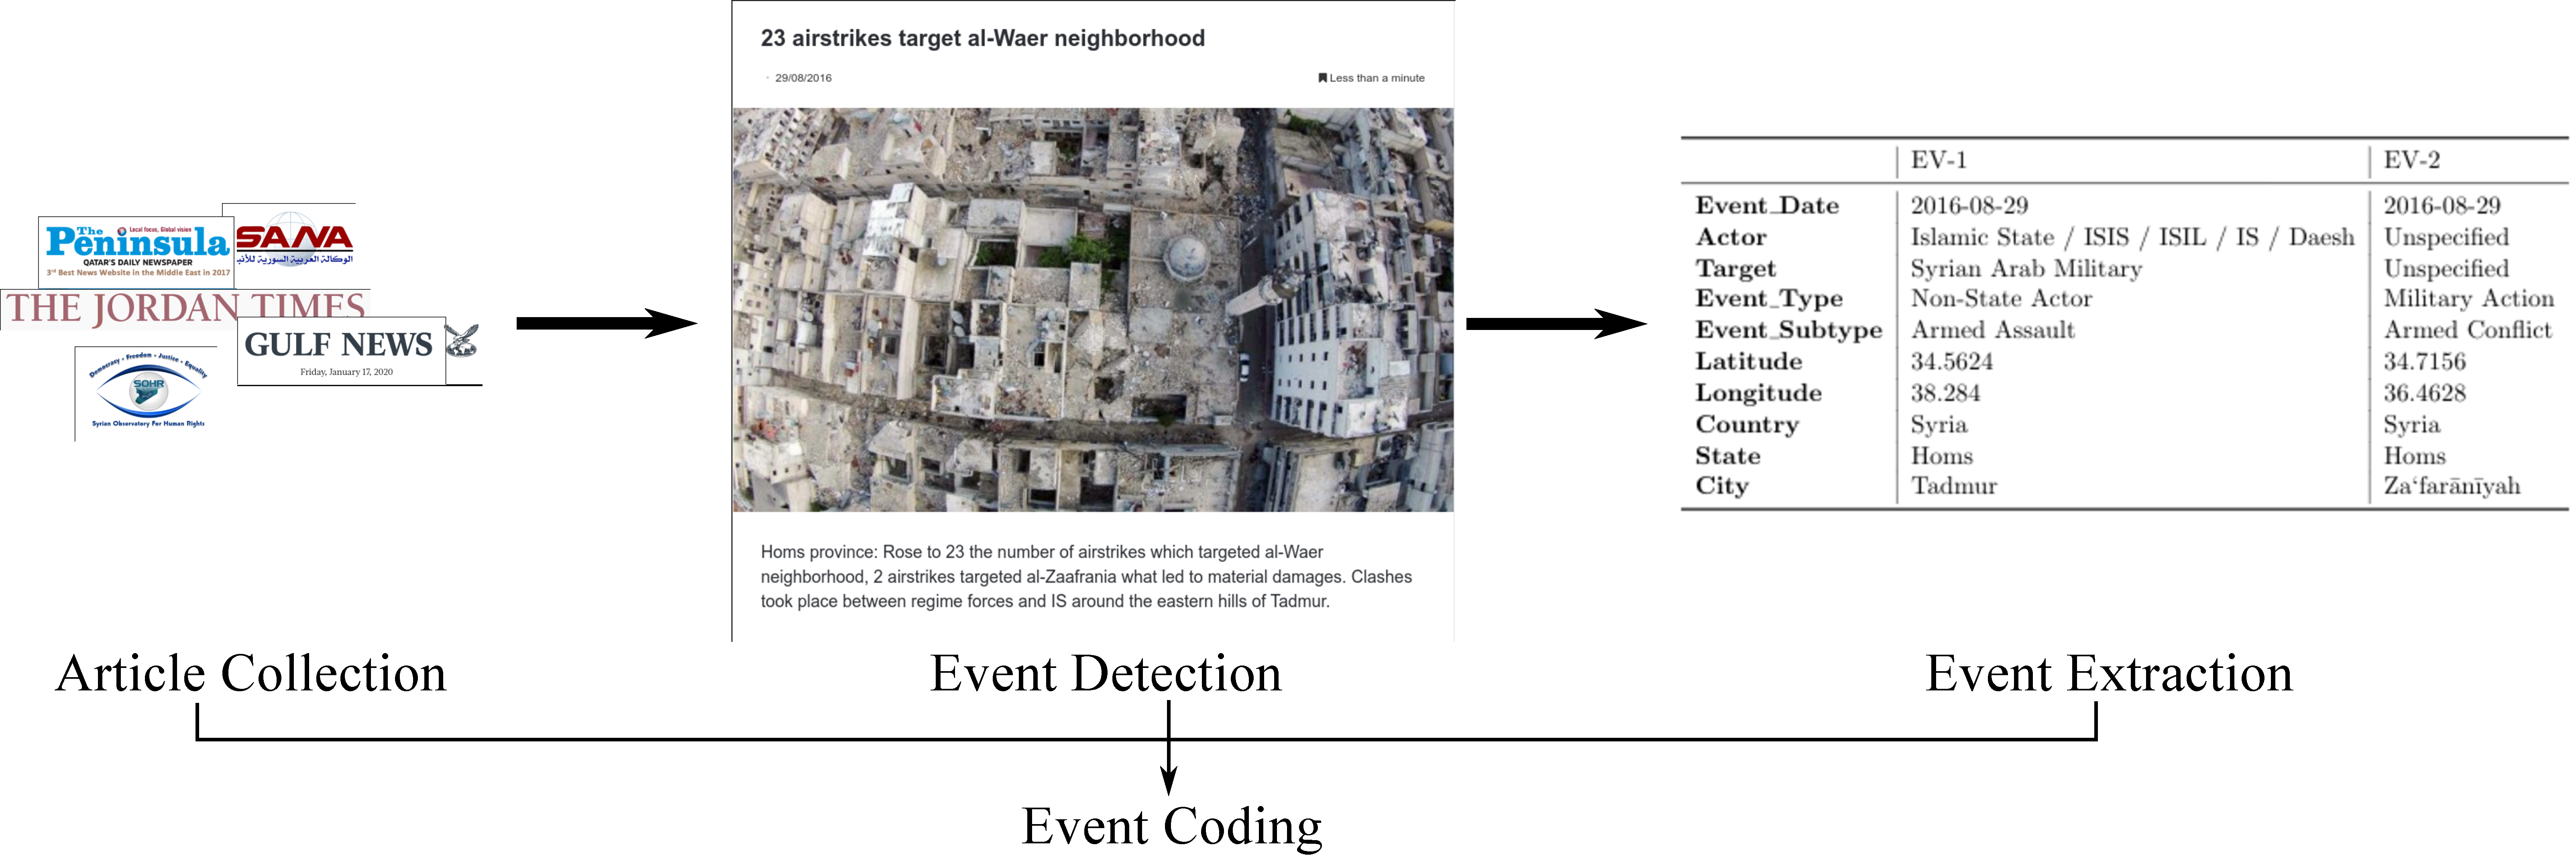
\includegraphics[width=\textwidth]{Problem2/figures/EventCoding_intro.pdf}
        \label{fig:my_label}
    \end{figure}
\end{frame}


%%\subsection{Necessity for a new Event Coder}
\begin{frame}{Necessity for a new Event Coder}
\begin{itemize}
    \item Manual event coders
    \begin{itemize}
        \item  High delay (OSI GSR (Goal Standard Report) had 1 month delay)
        \item High cost
    \end{itemize}
    \item Fully Automated Event coders 
    \begin{itemize}
        \item ICEWS~\cite{boschee2015icews}, GDELT~\cite{leetaru2013gdelt}
        \item Fixed dictionary (domain keywords and actors)
        \item fixed patterns for matching
        \item high duplicate levels
        \item Only English
    \end{itemize}
    \item Semi-Automatic event coders 
    \begin{itemize}
        \item EMBERS AutoGSR~\cite{saraf2016embers}
        \item Manual checking necessary for all fields and for all documents
    \end{itemize}
\end{itemize}
\end{frame}

%\subsection{Micro-tasks for Event Coding}
\begin{frame}{Micro-tasks for Event Coding}
    \begin{itemize}
    \item \textbf{Event Detection}: Classify if a news article is reporting an event of interest or not.
    \item \textbf{Geo-coding}: Identify and disambiguate location names from text
    \item \textbf{Actor / Target Linking}: Identify entities mentioned and link them to known actors. 
    \item \textbf{Temporal Reasoning}: Identify the exact date in which an event took place by resolving all direct and relative dates mentioned in the text.
    \item \textbf{Sub-type Identification}: This could be either the reason for the event (like Economic, Religious) in case of civil unrest or the kind of event (like bombing, hostage taking) in case of MANSA.
    \item \textbf{Event De-duplication}: Task of identifying if the current article refers to an already extracted event.
\end{itemize}
\end{frame}


%\subsection{System Framework}
\begin{frame}{System Framework}
    \begin{figure}
        \centering
        \includegraphics[width=\textwidth]{Problem2/figures/eventCoding_framework.pdf}
        \label{fig:my_label}
    \end{figure}
\end{frame}

%\subsection{Event Detection}
\begin{frame}{Event Detection}
Performed as a binary classification problem \\
\textbf{Uncertainty in Event Detection}
\begin{itemize}
    \item Base Classifier: Hierarchical Attention Network ~\cite{yang2016hierarchical}
    \item Uncertainty in Classification in literature
    \begin{itemize}
        \item Classification with reject option, Abstaining Classifiers, Selective classification 
        \item Methods can be broadly categorized into
        \begin{itemize}
            \item External model calibration - Platt scaling, Temperature scaling
            \item Ensemble learning - McDropout, Gaussian Process, Metric learning
            \item Learning a `K+1`th class for a K class problem - Deep.Abs Classifier, Evidential classification
        \end{itemize}
    \end{itemize}
    \end{itemize}
\end{frame}

\begin{frame}{Extraction using Dependency parsing}
\begin{itemize}
\small
    \item Extract events based on patterns on dependency tree
    \begin{itemize}
    \small
        \item ~\cite{predpatt},~\cite{pp-paper1},~\cite{reddy2017universal}
        \item universal dependency parser allows usage of same patterns for all languages
        \item All locations mentioned in the same sentence as the predicate-argument root is taken as Event location
    \end{itemize}    
\end{itemize}
\vspace{-1em}
\begin{figure}
    \centering
    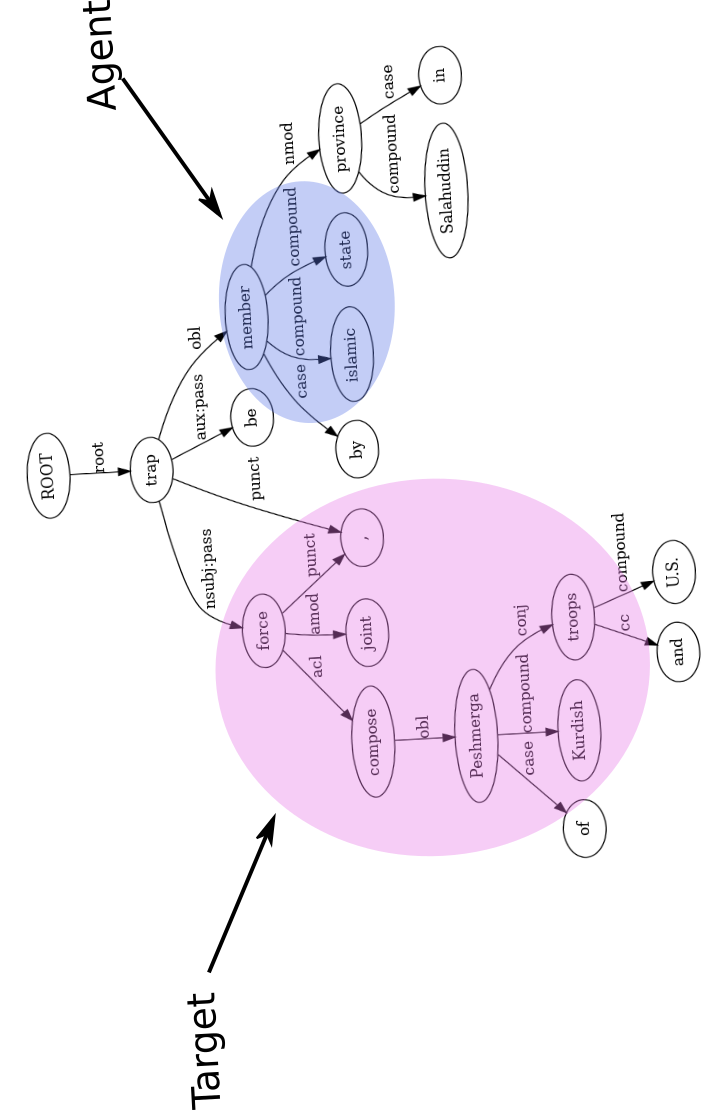
\includegraphics[width=0.35\textwidth, angle=-92]{Problem2/figures/depTree.png}
    \caption{Caption}
    \label{fig:my_label}
\end{figure}
\end{frame}

%\subsection{Geo-coding}
\begin{frame}{Geo-coding}
    Defined as the problem of identifying 1) mentions of placenames  in text and 2) grounding location names to geo-coordinates \\
    
    \begin{block}{Example}
    \alert{Baghdad Today} quoted the source saying that a bomb placed near a fish market in \alert{Wardiya, Madaen} exploded, killing one person and wounding four others
    \end{block}
\end{frame}

\begin{frame}{Geo-coding (contd.)}
\begin{itemize}
    \item Prior work is generally unsupervised and rule based
    \begin{itemize}
        \item Placenames are grounded to the most populous expansion (\textless Country, State, City \textgreater)
        \item Locations mentioned in same text share common ancestors or are nearby
    \end{itemize}
    \item Current state-of-the art - Mordecai~\cite{halterman2017mordecai}
    \begin{itemize}
        \item Neural network based model for inferring country for each placename
    \end{itemize}
\end{itemize}
\end{frame}

\begin{frame}{Supervised Geo-coding}

\begin{columns}
\column{0.6\textwidth}
Building Training Data

    \begin{itemize}
    \small
        \item Use only articles that contain events
        \item Extract placenames from article that have anyone grounding match to an event
        \item Expansion matching event location is labelled positive and rest negative
        \item Features
        \begin{itemize}
            \item Frequency of country in expansions of all names in text
            \item Relative Population 
            \item Mean, Min token distance to Placename having an expansion from the same country
            \item Token distance to the next nearest Placename (before and after)
        \end{itemize}
    \end{itemize}


\column{0.4\textwidth}
\begin{figure}
    \centering
    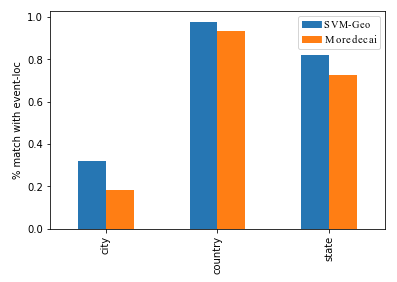
\includegraphics[width=\textwidth]{Problem2/figures/Geo_metrics.png}
    \label{fig:my_label}
\end{figure}
\end{columns}

\end{frame}

\begin{frame}{Uncertainty in Geo-coding}
\begin{itemize}
    \item Approximate locations
    \begin{itemize}
        \item Percentage of Approximate locations is 27.81\% (4400 events, 3053 documents, 5 month period)
        \begin{block}{}
         Three people killed by a landmine explosion in their car in the \alert{rough neighborhood of Jaroud Arsal} left behind by terrorists.
        \end{block}
        \item Uncertainty in Location disambiguation (Example on next slide)
    \end{itemize}
\end{itemize}
\end{frame}

\begin{frame}{Uncertainty in Geo-coding}
\begin{figure}
    \centering
    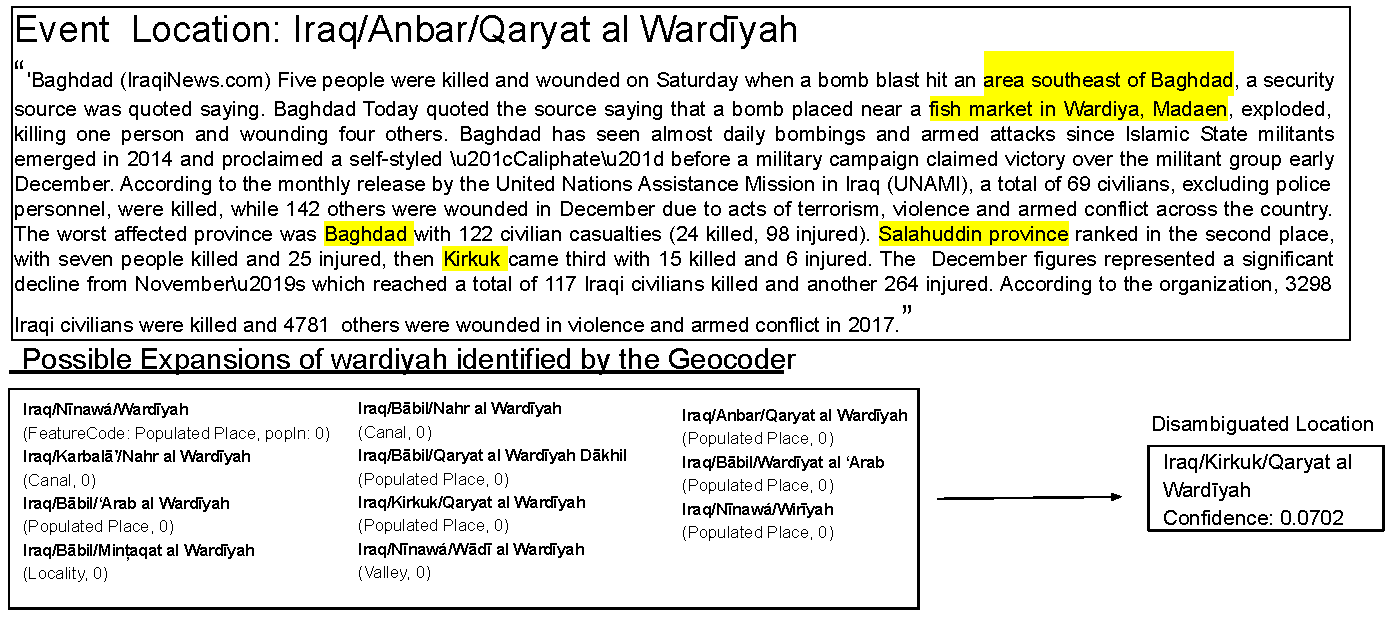
\includegraphics[width=1\textwidth]{Problem2/figures/Geo_uncertainty.pdf}
    \label{fig:my_label}
\end{figure}
\end{frame}

%\subsection{Actor/Target Linking}
\begin{frame}{Actor/Target Linking}
Categorized into two kinds
    \begin{itemize}
        \item Specific Nouns (like Jordanian Police, Democratic Union Party / PYD)
        \begin{itemize}
            \item Fuzzy token similarity for matching
        \end{itemize}
        \item Generic Nouns (Weapon/Equipment, Vehicle, Checkpoint)
        \begin{itemize}
            \item Expand keyword list
            \begin{itemize}
                \item High similarity neighbors from word embedding
                \item Example: Airstrike, bombardment
                \item Words that share similar hypernyms / hyponyms / synsets from Wordnet 
                \item Example: Builders, Contractors, Constructor
            \end{itemize}
        \end{itemize}
    \end{itemize}
\end{frame}

\begin{frame}{Uncertainty in Actor/Target Linking}
\begin{block}{EVENT:(Location) Syria-Aleppo-Rā‘il,  (Actor) Al-Moatasim / Al-Moatasim Brigade,  2018-05-23,  (Target) Unspecified}
\small
``The town of Al-Ra’I on the border with Turkey, which is controlled by the factions operating within the Turkish-backed operation of the “Euphrates Shield”, witnessed tension between a faction operating in the area and the free police operating in the town, and in the details obtained by the Syrian Observatory of Human Rights; the town is witnessing a state of alertness and tension, followed a fight took place between \alert{Al-Muntasir Brigade} against the free police, in the market of the town... ''
\end{block}

\begin{itemize}
    \item New Actor
    \item Unknown alias of an existing actor
\end{itemize}

\end{frame}

%\subsection{Temporal Resolution}
\begin{frame}{Temporal Resolution}
Broadly defined as the task of converting relative temporal expressions like `two days ago' into exact dates
\begin{itemize}
    \item TIMEN~\cite{timen}
    \item Heideltime~\cite{heideltime}
        \begin{itemize}
            \item Larger number of language classes
            \item Covers more temporal patterns
        \end{itemize}
\end{itemize}
\end{frame}



%\subsection{Sub-type Identification}
% \begin{frame}{Event Sub-type identification}
% \begin{itemize}

%     \item Word-net expansion and classification
%     \end{itemize}
% \end{frame}



%\subsection{Performance Metrics}
\begin{frame}{Performance Metrics}
Train Data: Upto May 2018, Validation: June 2018, Test - August-October 2018
\begin{itemize}
    \item \textbf{Event Detection Performance Metrics}
    \begin{itemize}
        \item Precision/Recall/F1 metrics
        \item Risk-Coverage Curve
        \begin{itemize}
            \item Risk is percentage of false classifications (False Positives + False Negatives)
            \item Coverage is percentage of data remaining after removing low-confidence documents
        \end{itemize}
    \end{itemize}
\item \textbf{Event Encoding Performance Metrics}
    \begin{itemize}
        \item \textbf{Quality Score:}  The components of QS are:
            \begin{enumerate}
                \item Actor score (AS)
                \item Target Target score (TTS)
                \item Target Status score (TS)
                \item Location score (LS): $(1 – Dist/300)$
                \item Event Sub-type score (ES)
                \item Date score (DS): $max(diff, 7)/7$
            \end{enumerate}
         \item \textbf{Macro and Micro averages}
    \end{itemize}    
\end{itemize}
\end{frame}


\begin{frame}{Event Detection Performance}
\textbf{English}
\begin{table}
\small
    \centering
   \begin{tabular}{lrrrr}
\toprule
{} &  Precision &  Recall &    F1-score &  Support \\
\midrule
No-event            &  0.97 &   0.95 &  0.96 &   15843 \\
Event               &  0.75 &   0.84 &  0.79 &   2760 \\
micro avg           &  0.93 &   0.93 &  0.93 &   18603 \\
macro avg           &  0.86 &   0.90 &  0.88 &   18603 \\
weighted avg        &  0.94 &   0.93 &  0.94 &   18603 \\
\bottomrule
\end{tabular}
    \label{tab:engDetection}
\end{table}

\textbf{Arabic}
\begin{table}
\small
    \centering
   \begin{tabular}{lrrrr}
\toprule
{} &  Precision &  Recall &    F1-score &  Support \\
\midrule
No-event            &  1.0 &  1.00 &  1.00 &  28643 \\
Event               &  1.0 &  0.36 &  0.53 &   73 \\
micro avg           &  1.0 &  1.00 &  1.00 &  28716 \\
macro avg           &  1.0 &  0.68 &  0.76 &  28716 \\
weighted avg        &  1.0 &  1.0  &  1.00 &  28716 \\
\bottomrule
\end{tabular}
    \label{tab:arDetection}
\end{table}
\end{frame}

\begin{frame}{Performance of fully Automated system}
\begin{columns}
\column{0.3\textwidth}
\textbf{Macro-Avg}: Extracted events in a document are only evaluated against the ground-truth events in that document
\column{0.7\textwidth}
        \begin{table}
    \centering
    \begin{tabular}{l|r|r}
    \toprule
                 Metrics &    Macro-avg &    Micro-avg \\
    \midrule
                   \#docs &   888 &   888 \\
     \# GroundTruthEvents &  2039 &  2039 \\
       \# ExtractedEvents &  1981 &  1981 \\
             Actor Score &     0.373888 &     0.602880 \\
              Date Score &     0.940764 &     0.840740 \\
     Event Subtype Score &     0.449895 &     0.680532 \\
          Location Score &     0.866620 &     0.800837 \\
     Target Target Score &     0.662297 &     0.677204 \\
     Target Status Score &     0.590778 &     0.828618 \\
               Precision &     0.691522 &     0.949447 \\
                  Recall &     0.720177 &     0.891757 \\
           Quality Score &     2.774264 &     2.999131 \\
    \bottomrule
    \end{tabular}
    \label{tab:mlPerformance}
    \end{table}
\end{columns}
\end{frame}

\begin{frame}{System Performance after Actor Grouping}
\begin{columns}
\column{0.5\textwidth}
\begin{itemize}
    \item Group different state actors of a given country into one entity
    \item Example: Following are grouped into Iraqi State Actors
    \begin{itemize}
        \item Iraq Security Forces
        \item Iraqi Intelligence Service
        \item Iraqi Police
        \item Baghdad International Airport Security
        \item Iraqi Military
        \item Iraqi Special Forces
    \end{itemize}
\end{itemize}
\column{0.5\textwidth}
\begin{table}
\centering
\begin{tabular}{lrr}
\toprule
       Metric &    Macro-avg &    Micro-avg \\
\midrule
\textbf{After} & & \\
       AS &     0.551 &     0.727 \\
       QS &     2.892 &     3.087 \\
       \midrule
       \textbf{Before} & & \\
        AS &     0.373 &     0.602 \\
        QS &     2.774 &     2.999 \\
\bottomrule
\end{tabular}
\label{tab:mlgrouped}
\end{table}
\end{columns}
\end{frame}

\begin{frame}{Characterization of human annotators}
\begin{figure}
     \centering
     \begin{subfigure}[b]{0.5\textwidth}
         \centering
         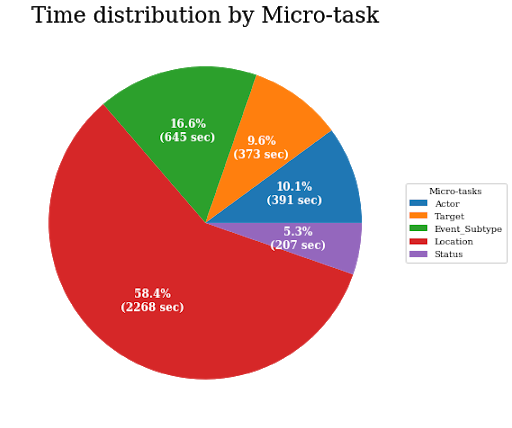
\includegraphics[width=\textwidth]{Problem2/figures/micro_task_timings.png}
     \end{subfigure}%
     \hfill
     \begin{subfigure}[b]{0.5\textwidth}
         \centering
         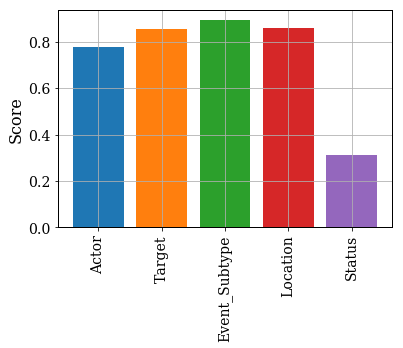
\includegraphics[width=\textwidth]{Problem2/figures/micro_task_performance.png}
     \end{subfigure}
\end{figure}
    
\end{frame}

% \begin{frame}{Uncertainty characterization event detection model}
% \begin{col}
% \begin{figure}
%     \centering
%     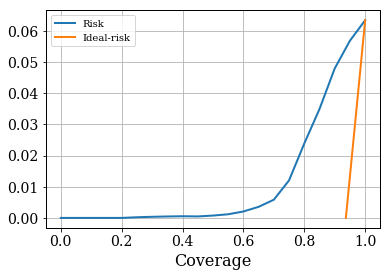
\includegraphics[width=0.45\textwidth]{Problem2/figures/english_riskCoverage.png}
% \end{figure}
% \end{frame}

\begin{frame}{Number of Documents sent for supervision}
\begin{table}
    \centering
    \small
    \begin{tabular}{l|r}
    \toprule
       \textbf{Micro-Task}  & \textbf{\#Abstained Documents} \\
    \midrule
       Event Detection &  1936 / 57401 (3.00\%) \\
       Location  & 307/2137 (14.3\%) \\
       Actor/Target & 1002/2137 (46.8\%) \\
       All (Location, Actor, Subtype) & 320/2137 (14.9\%) \\
    \bottomrule
    \end{tabular}
    \caption{Documents sent for human supervision}
    \label{tab:abstPerMicro}
\end{table}
\end{frame}

\begin{frame}{Performance of Hybrid System}
    \begin{table}[]
    \centering
    \begin{tabular}{lrr}
\toprule
              Metric &    Macro-avg &    Micro-avg \\
\midrule
               \#docs &  2137 &  2137 \\
 \# GroundTruthEvents &  4265 &  4265 \\
   \# ExtractedEvents &  4239 &  4239 \\
         Actor Score &     0.621032 &     0.755090 \\
          Date Score &     0.952899 &     0.878390 \\
 Event Subtype Score &     0.539359 &     0.646776 \\
      Location Score &     0.926107 &     0.838040 \\
 Target Target Score &     0.680881 &     0.703337 \\
 Target Status Score &     0.727046 &     0.828054 \\
           Precision &     0.791948 &     0.946720 \\
              Recall &     0.819668 &     0.915887 \\
       Quality Score &     3.121909 &     3.161470 \\
\bottomrule
\end{tabular}
    \label{tab:hybridPerf}
\end{table}
\end{frame}

\begin{frame}{Comparison with ICEWS}
CAMEO Codes used: 1) 15 - Exhibit Military Posture,  2) 18 - Assault
\begin{figure}
    \centering
    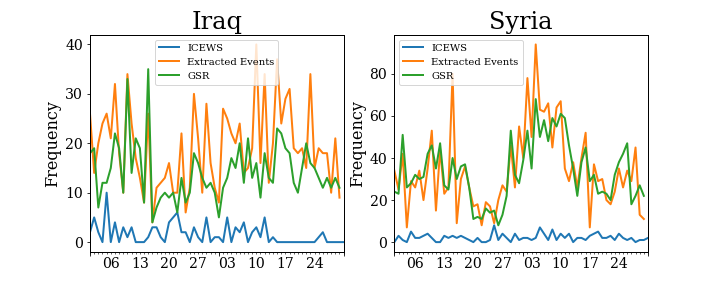
\includegraphics[width=\textwidth]{Problem2/figures/ICEWS_comparison.png}
\end{figure}
    
\end{frame}

\begin{frame}{Takeaways}
\begin{itemize}
    \item Automated methods perform well in identifying Location, Date
    \item Human supervision necessary for Actor/Target identification
    \item Contributions
    \begin{itemize}
        \item Improved geo-coding performance
        \item Automated approaches for keyword expansion
        \item language agnostic extraction
    \end{itemize}
\end{itemize}
    
\end{frame}



% % \section{Problem 3}
% % \begin{frame}{Uncertainty in Classification}
    Define sources of uncertainty
\end{frame}

\begin{frame}{Current State-of-the-art}
    List all related work
\end{frame}

\begin{frame}{Proposed Idea}
    
\end{frame}



%% \section{Proposed Problems}
\section{Uncertainty Aware Multi-instance Learning for Event Detection}
\begin{frame}{Uncertainty Aware Multi-instance Learning for Event Detection}
\begin{itemize}
    \item Can we highlight what text is responsible for the increased uncertainty of a document?
    \begin{itemize}
        \item Most existing work are black-box
        \item Highlighting uncertain text will help
            \begin{itemize}
                \item Reduce human time spent in analyzing the entire document text
                \item Identify which kind of documents/text we need more supervision for
            \end{itemize}
    \end{itemize}
\end{itemize}
\begin{small}
\begin{block}{Example}
BEIRUT , LEBANON ( 2:00 A.M. ) – A large number of Syrian military reinforcements reportedly arrived in the western countryside of the Idlib Governorate recently , as they prepare to launch an offensive in the Al - Ghaab Plain and Jisr Al - Shughour District
Pro - opposition accounts and Hay’at Tahrir Al - Sham ’s official media wing \alert{claimed on Tuesday that the Syrian military had sent reinforcements} to the Al - Ghaab Plain to launch an offensive in Syria.
\end{block}
\end{small}
\end{frame}

\begin{frame}{Uncertainty Aware Multi-instance Learning for Event Detection}
\begin{itemize}
    \item Multi-instance learning - Label information is available only at bag/group level
    \item A bag/group is positive if at-least one instance is positive
    \item Problem: Infer instance labels from group labels
\end{itemize}
    \begin{figure}
        \centering
        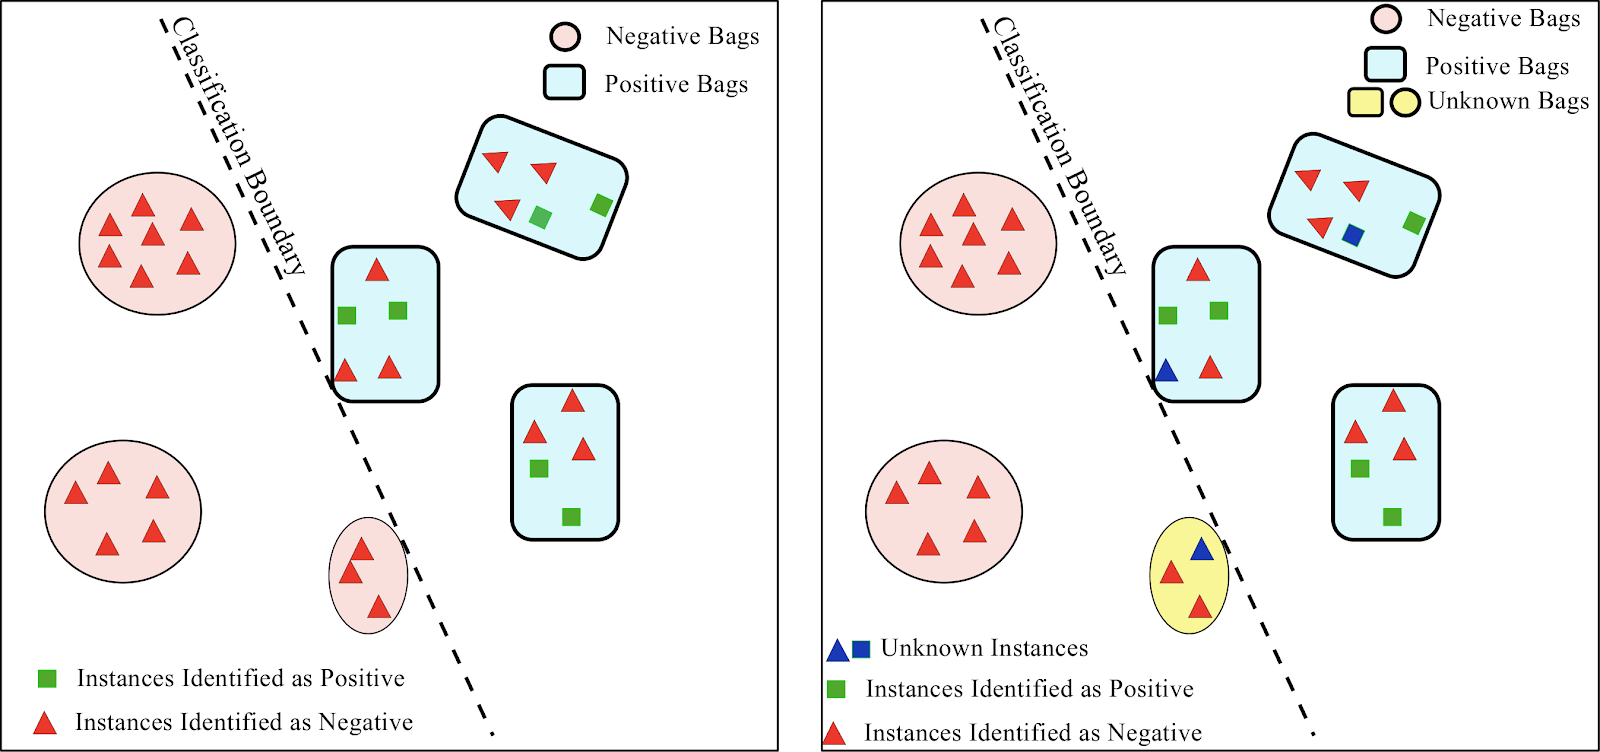
\includegraphics[width=0.75\textwidth]{Problem4/figures/MIL_kwik.png}
    \end{figure}
\end{frame}

\section{Reasoning over Event Progressions}
\begin{frame}{Reasoning over Event Progressions}
\begin{itemize}
    \item Event coders extract events independent of each other
        \begin{itemize}
            \item Does not take into account relation between events 
            \item A single event happening across multiple locations or over multiple days may be coded
            as multiple events due to limitation in event definition  (like CAMEO Ontology~\cite{schrodt2012cameo}) used by coders
        \end{itemize}
    \item Understanding if events belong to a bigger chain of events is important as it leads to improved situational awareness
    \begin{itemize}
        \item Example: Chain of protests regarding the 43 Missing students case
        \item Brazil spring protests
    \end{itemize}
\end{itemize}
\end{frame}
\begin{frame}{Example of Event Progression}
    \begin{figure}
        \centering
        \includegraphics[width=0.9\textwidth]{Problem4/figures/Matching&EventSignificance.pdf}
    \end{figure}
\end{frame}

\begin{frame}
    \begin{itemize}
    \item Understanding of event progressions and grouping helps
    \begin{itemize}
        \item Uncover hidden relations between supposedly unrelated events
        \item Allow an additional dimension of modeling and analysis
        \item identifying uncertain and missing events
    \end{itemize}
    
    \item Possible Approach - Temporal clustering of documents
        \begin{itemize}
                \item Storytelling~\cite{schlachter2015leveraging}
                \item document text is generally not available 
                    \begin{itemize}
                        \item URL's might become invalid over-time
                        \item Example: ICEWS, RavenPack etc
                    \end{itemize}
        \end{itemize}
\end{itemize}
\end{frame}

\begin{frame}{Reasoning over Event Progressions}
    \begin{itemize}
        \item Events can be viewed as Temporal Knowledge Graphs
    \end{itemize}
\begin{figure}
     \centering
     \begin{subfigure}[b]{0.5\textwidth}
         \centering
         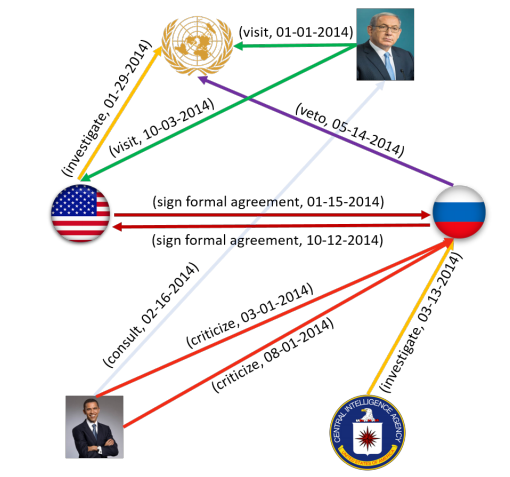
\includegraphics[width=0.5\textwidth]{Problem4/figures/know-evolve.png}
         \caption{~\cite{trivedi2017know}}
     \end{subfigure}%
     \hfill
     \begin{subfigure}[b]{0.5\textwidth}
         \centering
         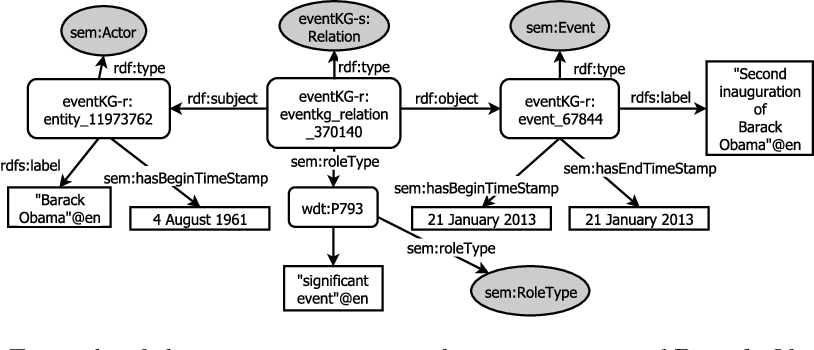
\includegraphics[width=0.8\textwidth]{Problem4/figures/EKG.png}
         \caption{~\cite{gottschalk2018eventkg}}
     \end{subfigure}
\end{figure}
\end{frame}

\section{Proposed Timeline}
\begin{frame}{Proposed Timeline}
\begin{figure}
    \centering
    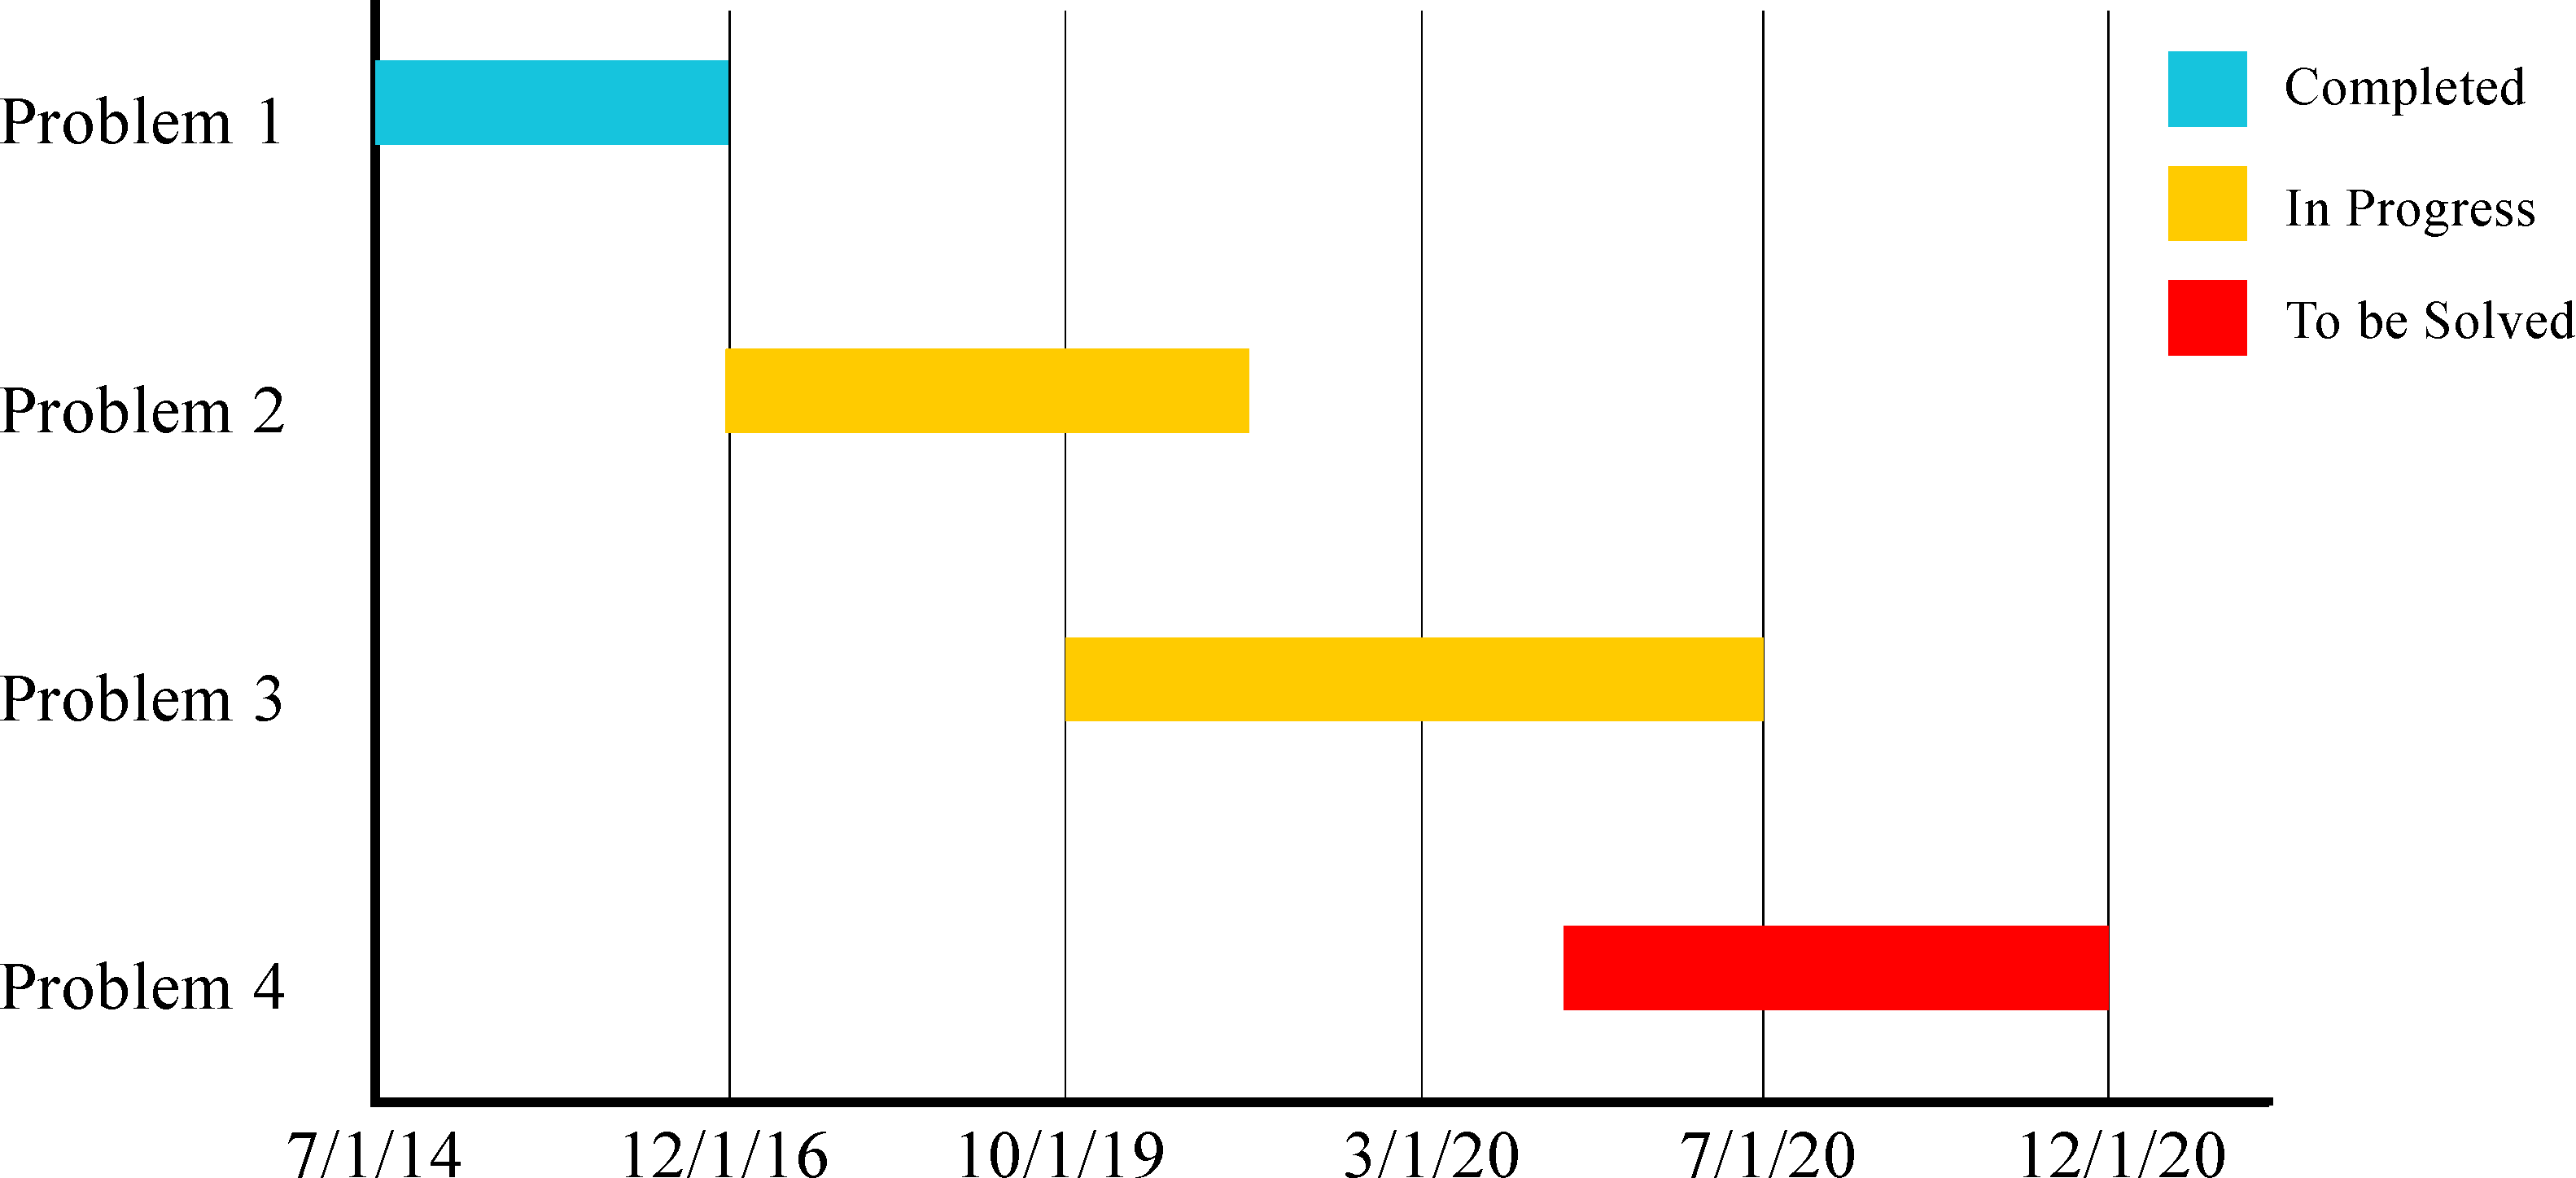
\includegraphics[width=\textwidth]{Problem4/figures/phdTimeline.pdf}
\end{figure}
\end{frame}

%% \section{Timeline}
% \begin{frame}{Proposed Timeline}
%     \begin{figure}
%         \centering
%         \includegraphics{}
%     \end{figure}
% \end{frame}

\begin{frame}{Publications}
\bibentry{Muthiah:2016:EYE:2939672.2939709}

\textbf{Other}\\
\begin{itemize}
    \item \bibentry{prottox}
    \item \bibentry{dyatsIJCAI}
    \item \bibentry{nactSeer}
    \item \bibentry{Ning:2016:MPE:2939672.2939802}
\end{itemize}
\end{frame}

\begin{frame}{Publications (Contd.)}
\textbf{Other} \\
\begin{itemize}
    \item \bibentry{kdd:beating-the-news}
    \item \bibentry{doyle2014forecasting} 
    \item \bibentry{chakraborty2016hierarchical}
\end{itemize}

\end{frame}


\begin{frame}[allowframebreaks]
        \frametitle{References}
        \bibliographystyle{apalike}
        \bibliography{references.bib}
\end{frame}

\begin{frame}{Uncertainty in Event Detection}
\begin{figure}
    \centering
    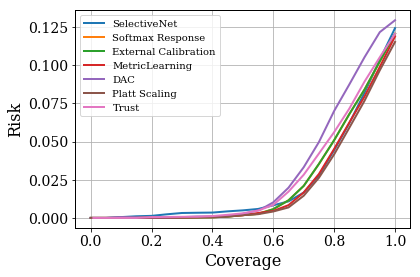
\includegraphics[width=0.5\textwidth]{Problem2/figures/Calibration_riskCoverage.png}    
\end{figure}
Coverage is defined as the percentage of data remaining after churning out documents on which the model score is less than the identified threshold. 

The curve is plotted by first sorting the model predictions in terms of its confidence score and moving the threshold from 0 to 100th percentile value of the confidence score. 

\end{frame}


\end{document}
